\documentclass[a4paper, 12pt, finnish]{article}
\usepackage{babel}
\usepackage[utf8]{inputenc}
\usepackage[T1]{fontenc}
\usepackage{graphicx}
\usepackage{caption}
\captionsetup{labelformat=empty}
\title{Keskustelufoorumin Dokumentaatio}
\author{Timo Mäki}
\date{\today}

\begin{document}
 \maketitle

Tämä on dokumentaatio tietokantasovelluksen harjoitustyön keskustelufoorumiin.

\newpage\null\thispagestyle{empty}\newpage
\tableofcontents
\newpage\null\thispagestyle{empty}\newpage
\section{Johdanto}

Aiheena on luoda keskustelufoorumi.
Foorumissa käyttäjät voivat kirjoittaa viestejä ja lukea muiden kirjoittamia viestejä.
Viestit liittyvät viestiketjuihin, joilla on otsikoita.
Käyttäjät voivat luoda viestiketjuja.
Viestejä tulee voida myös etsiä otsikon, iän tai kirjoittajan perusteella. Käyttäjillä on yksityiset tunnukset, joilla he voivat kirjautua sisään.
Tunnukset tarvitaan, jotta voi kirjoittaa viestin foorumille.
Jokaisella käyttäjätunnuksella voi kirjoittaa viestejä.
Pääkäyttäjällä on oikeus viedä käyttäjän oikeus kirjoittaa viestejä, sekä poistaa viestejä, että viestiketjuja.
\indent

Foorumin tarkoitus on edistää sosiaalista kanssakäyntiä ihmisten välillä, auttaa samanhenkisiä ihmisiä löytämään toisensa ja antaa ihmisten sekä anonyymisti että toisia kunnioittavasti esittää mielipiteitään internetin välityksellä.
\indent

Järjestelmän tavoitteet ovat mahdollistaa viestien kirjoitus ja luku, käyttäjätunnusten luonti, käyttöoikeus ryhmien olemassaolo sekä mahdollistaa nopea viestin haku.
\indent

Järjestelmä pyörii tktl:n users palvelimella, apachea käyttäen.
Se vaatii PHP-tuen.
Käyttäjän selaimelta ei edellytetä tukea javascriptille, mutta HTML5 tuki edellytetään.
Järjestelmä edellyttää PostgreSQL tietokantaa.
On todennäköistä, että, rajapintoja hyödyntäen, tietokanta tulee olemaan silti helppo vaihtaa.

\newpage
\section{Yleiskuva järjestelmästä}
\subsection{Jokamies}
Jokamies on henkilö, joka ei ole välttämättä rekisteröitynyt tai kirjautunut sisään.
Jokainen foorumin käyttäjä on jokamies.

\begin{itemize}
\item
Voi lukea foorumille tehtyjä kirjoituksia.

\item
Voi hakea viestejä.

\item
Voi rekisteröityä.

\item
Voi kirjautua foorumiin.
\end{itemize}

\subsection{Rekisteröitynyt käyttäjä}
Rekisteröitynyt käyttäjä on henkilö, joka on rekisteröinyt tunnuksen foorumille.

\begin{itemize}
\item
    Voi aloittaa uuden viestiketjun.
\item
    Voi vastata olemassa olevaan viestiketjuun.
\item
    Näkee kirjoitukset, joita henkilö ei ole vielä lukenut.
\end{itemize}

\subsection{Pääkäyttäjä}
Pääkäyttäjä on henkilö, joka vastaa foorumin ylläpidosta.
Tämä on erityisryhmä ja on oletusarvoisesti vain foorumin perustajalla. Pääkäyttäjällä on myös rekisteröityneen käyttäjän oikeudet.

\begin{itemize}
\item
Voi poistaa foorumille kirjoitetun viestin tai viestiketjun.
\item
Voi laittaa eston käyttäjälle, jolloin tämä ei voi enää kirjoittaa uusia viestejä foorumille.
\item
Voi antaa pääkäyttäjän oikeudet muille rekisteröityneille käyttäjille.
\end{itemize}

\newpage

\section{Käyttötapauskaavio}
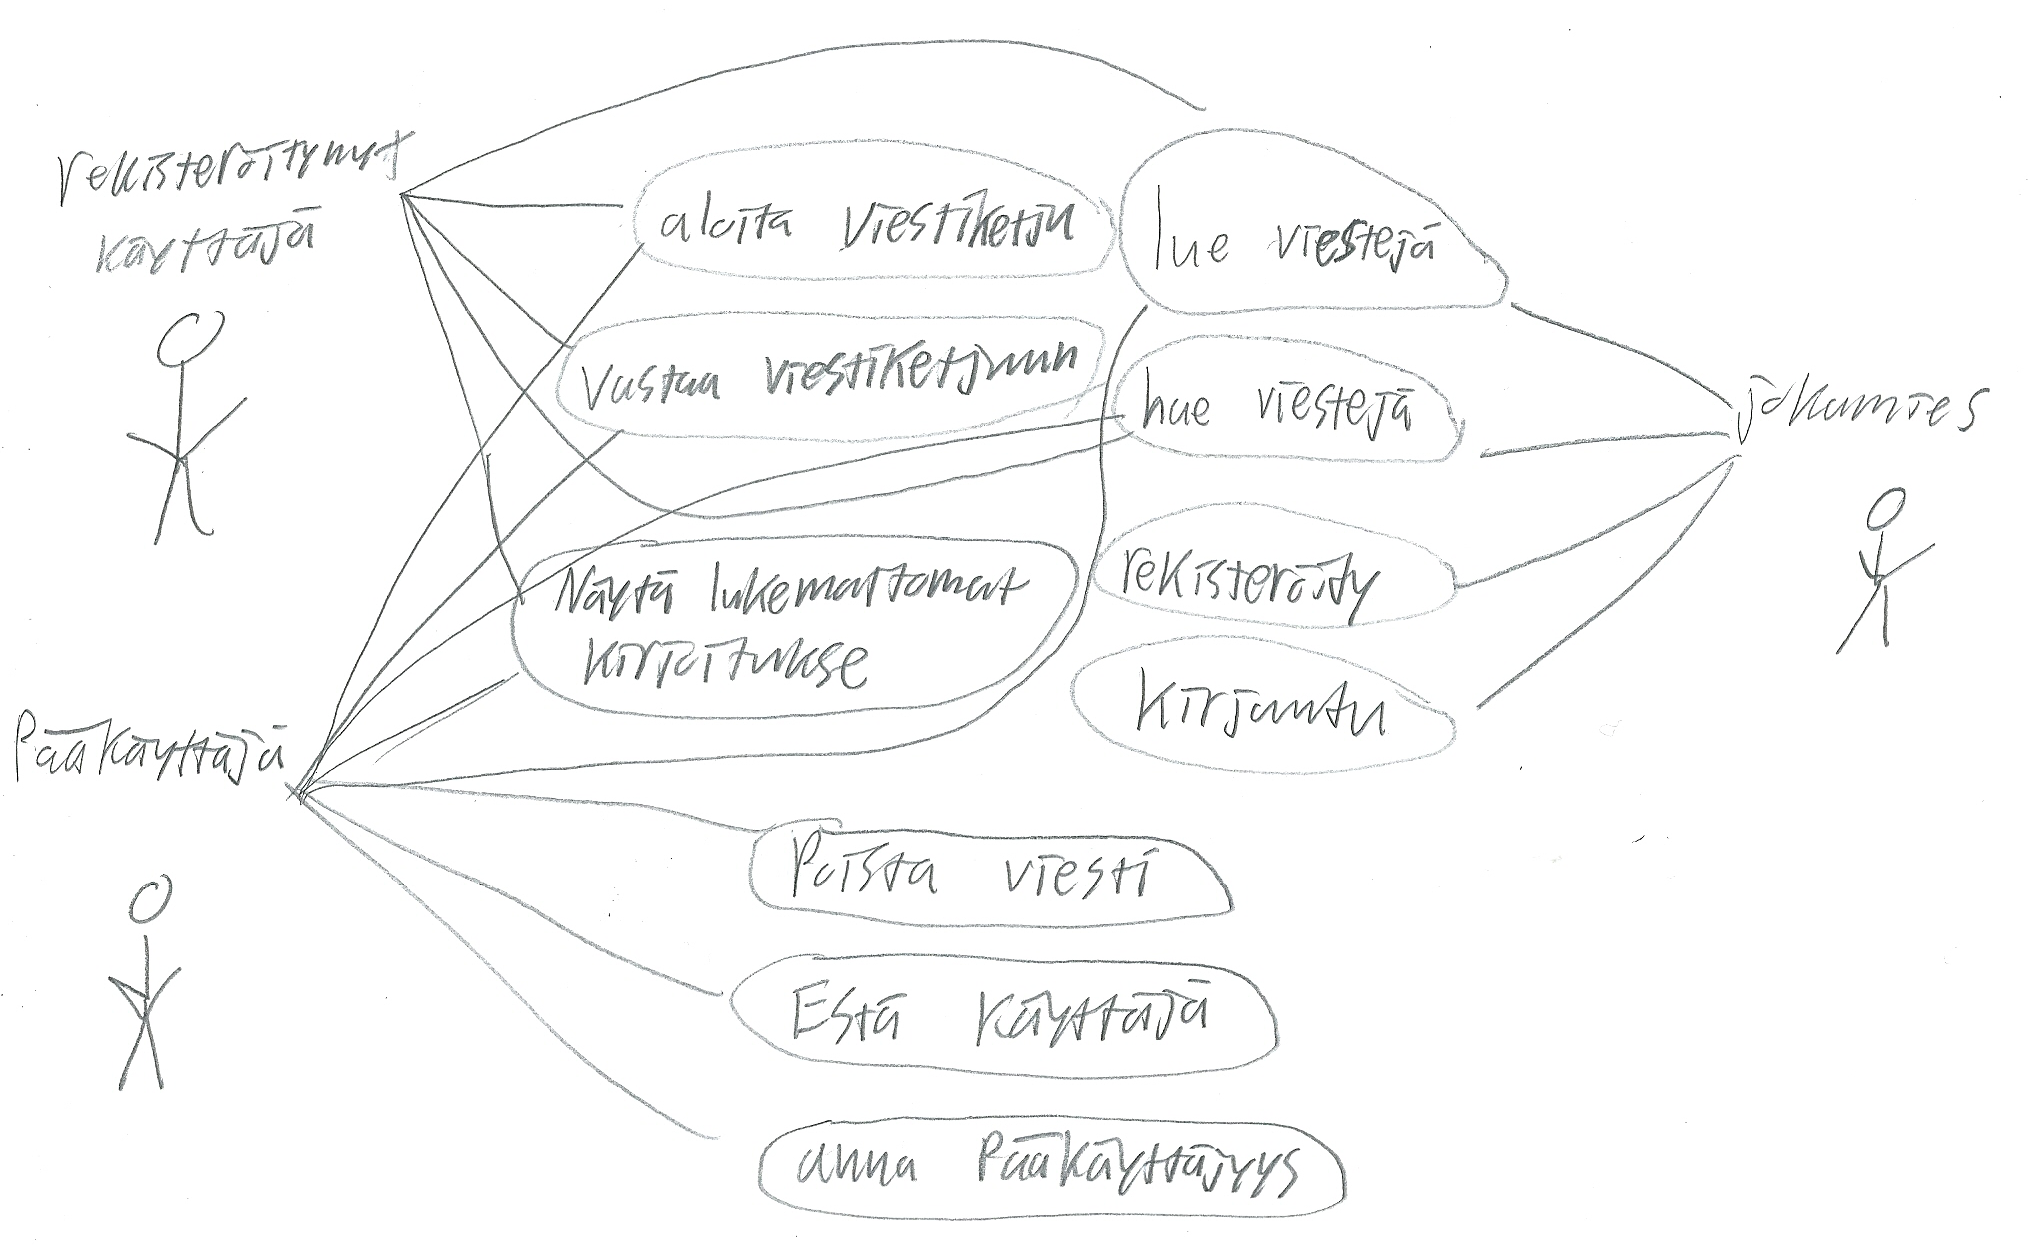
\includegraphics[width=\textwidth,height=\textheight,keepaspectratio]{kayttotapauskaavio.png}

\newpage

\section{Järjestelmän tietosisältö}
\subsection{Käsitekaavio}
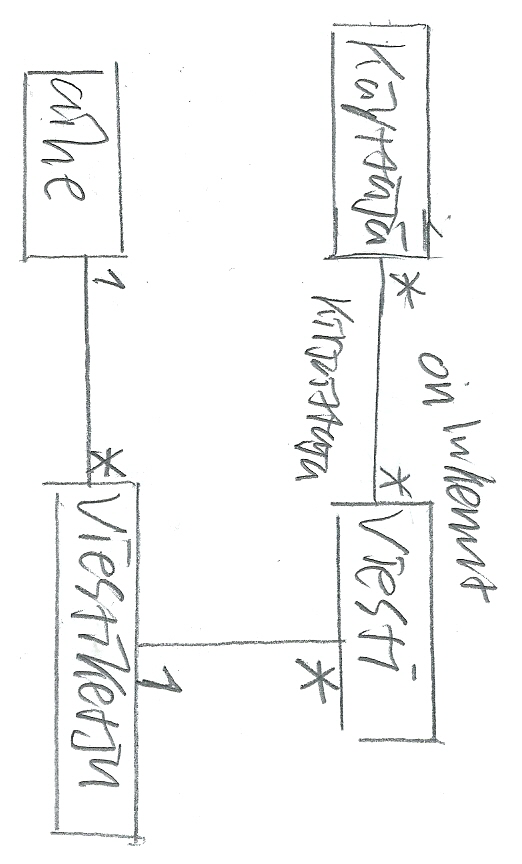
\includegraphics[width=\textwidth,height=\textheight,keepaspectratio]{kasitekaavio.png}

\subsection{Tietosisältö}
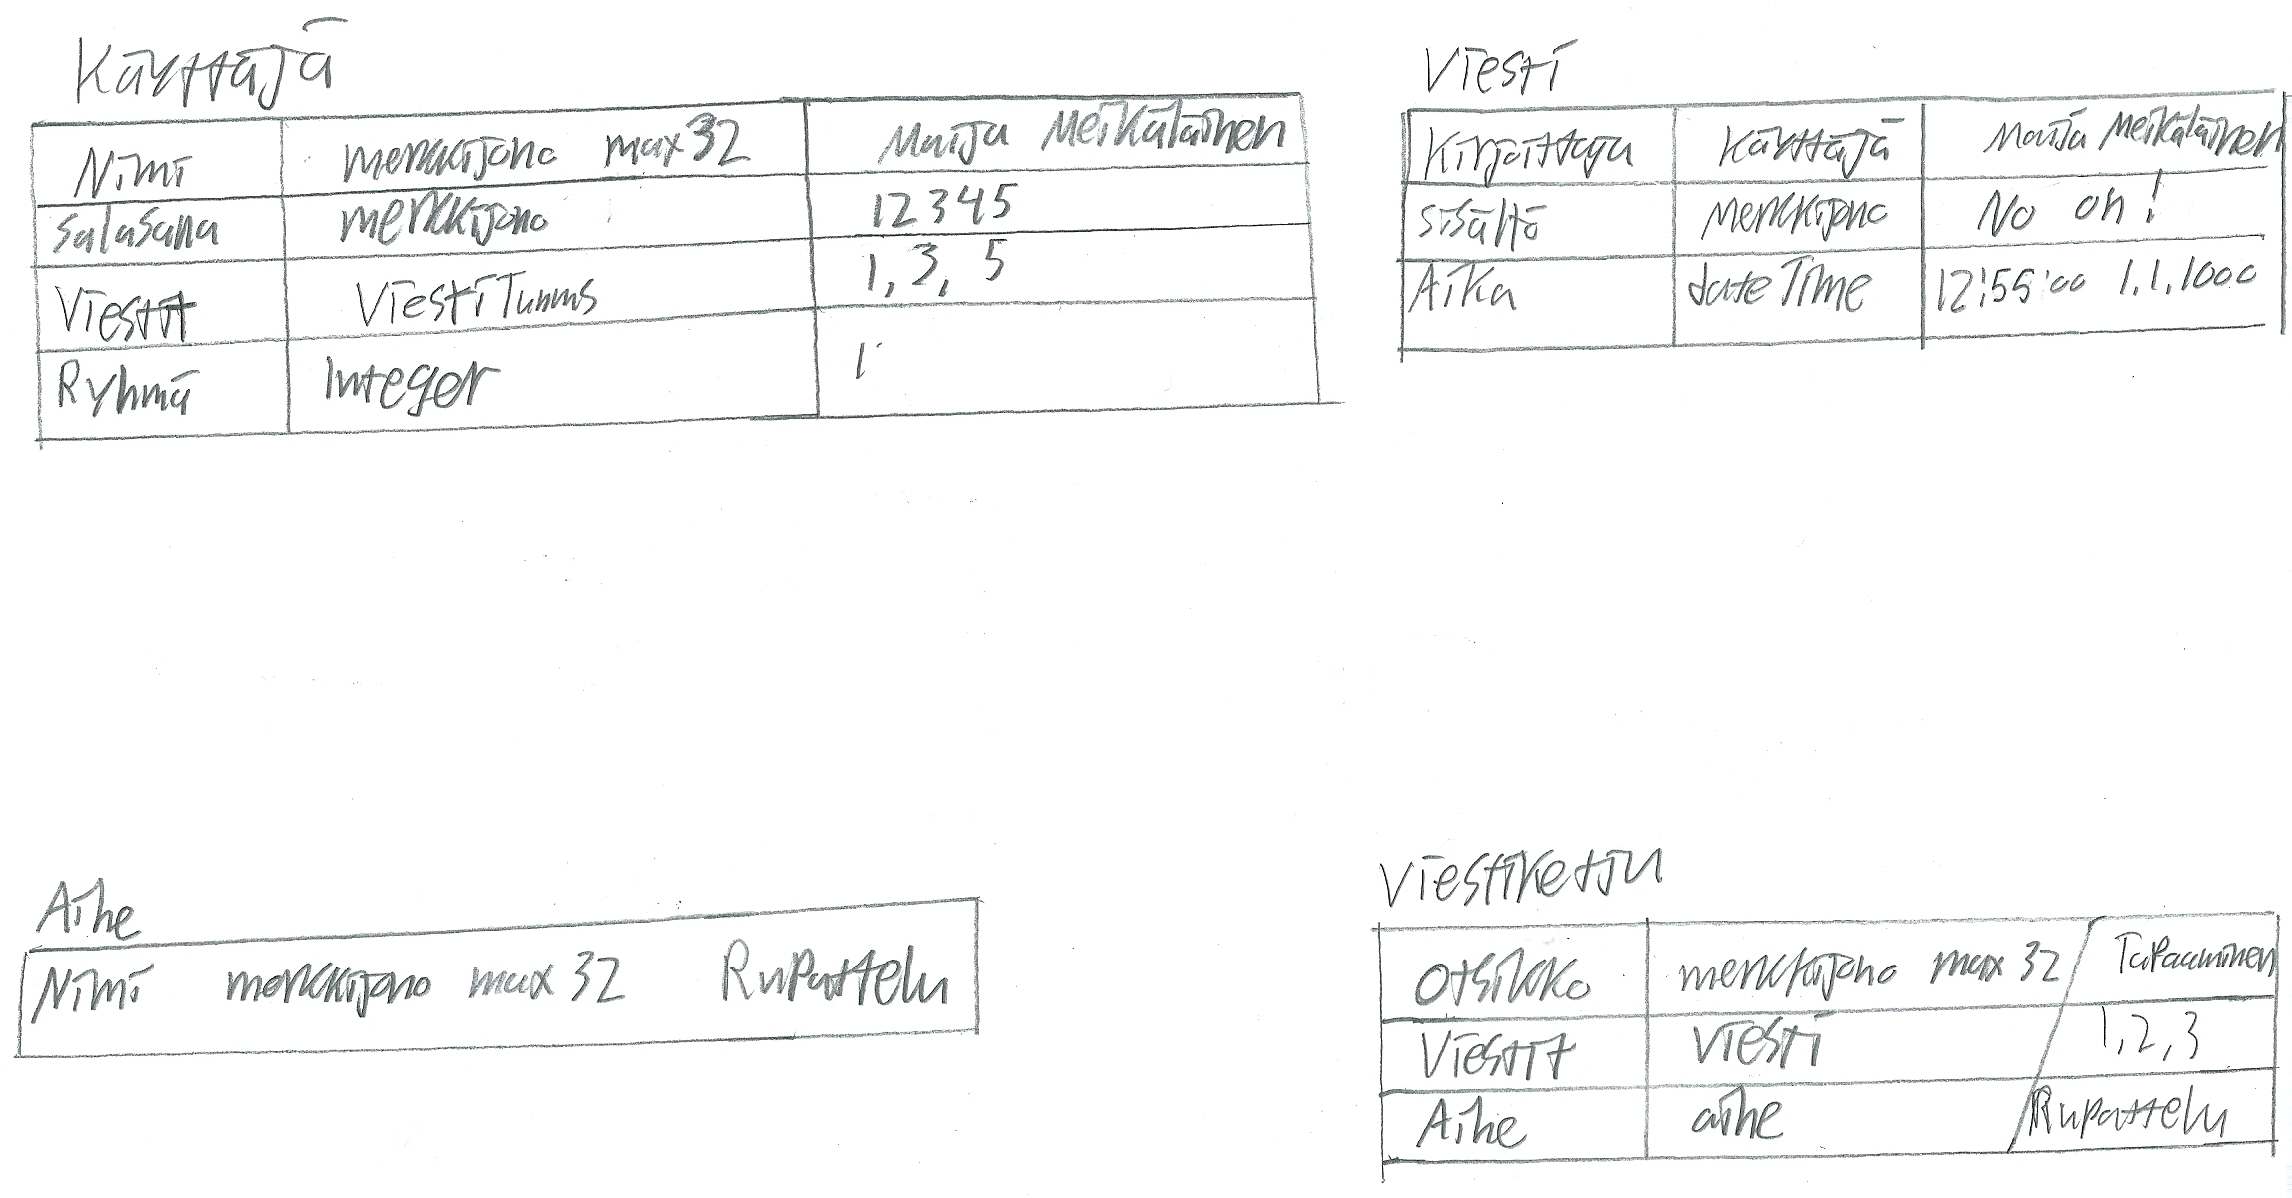
\includegraphics[width=\textwidth,height=\textheight,keepaspectratio]{tietosisalto.png}

\newpage

\section{Relaatiotietokantakaavio}
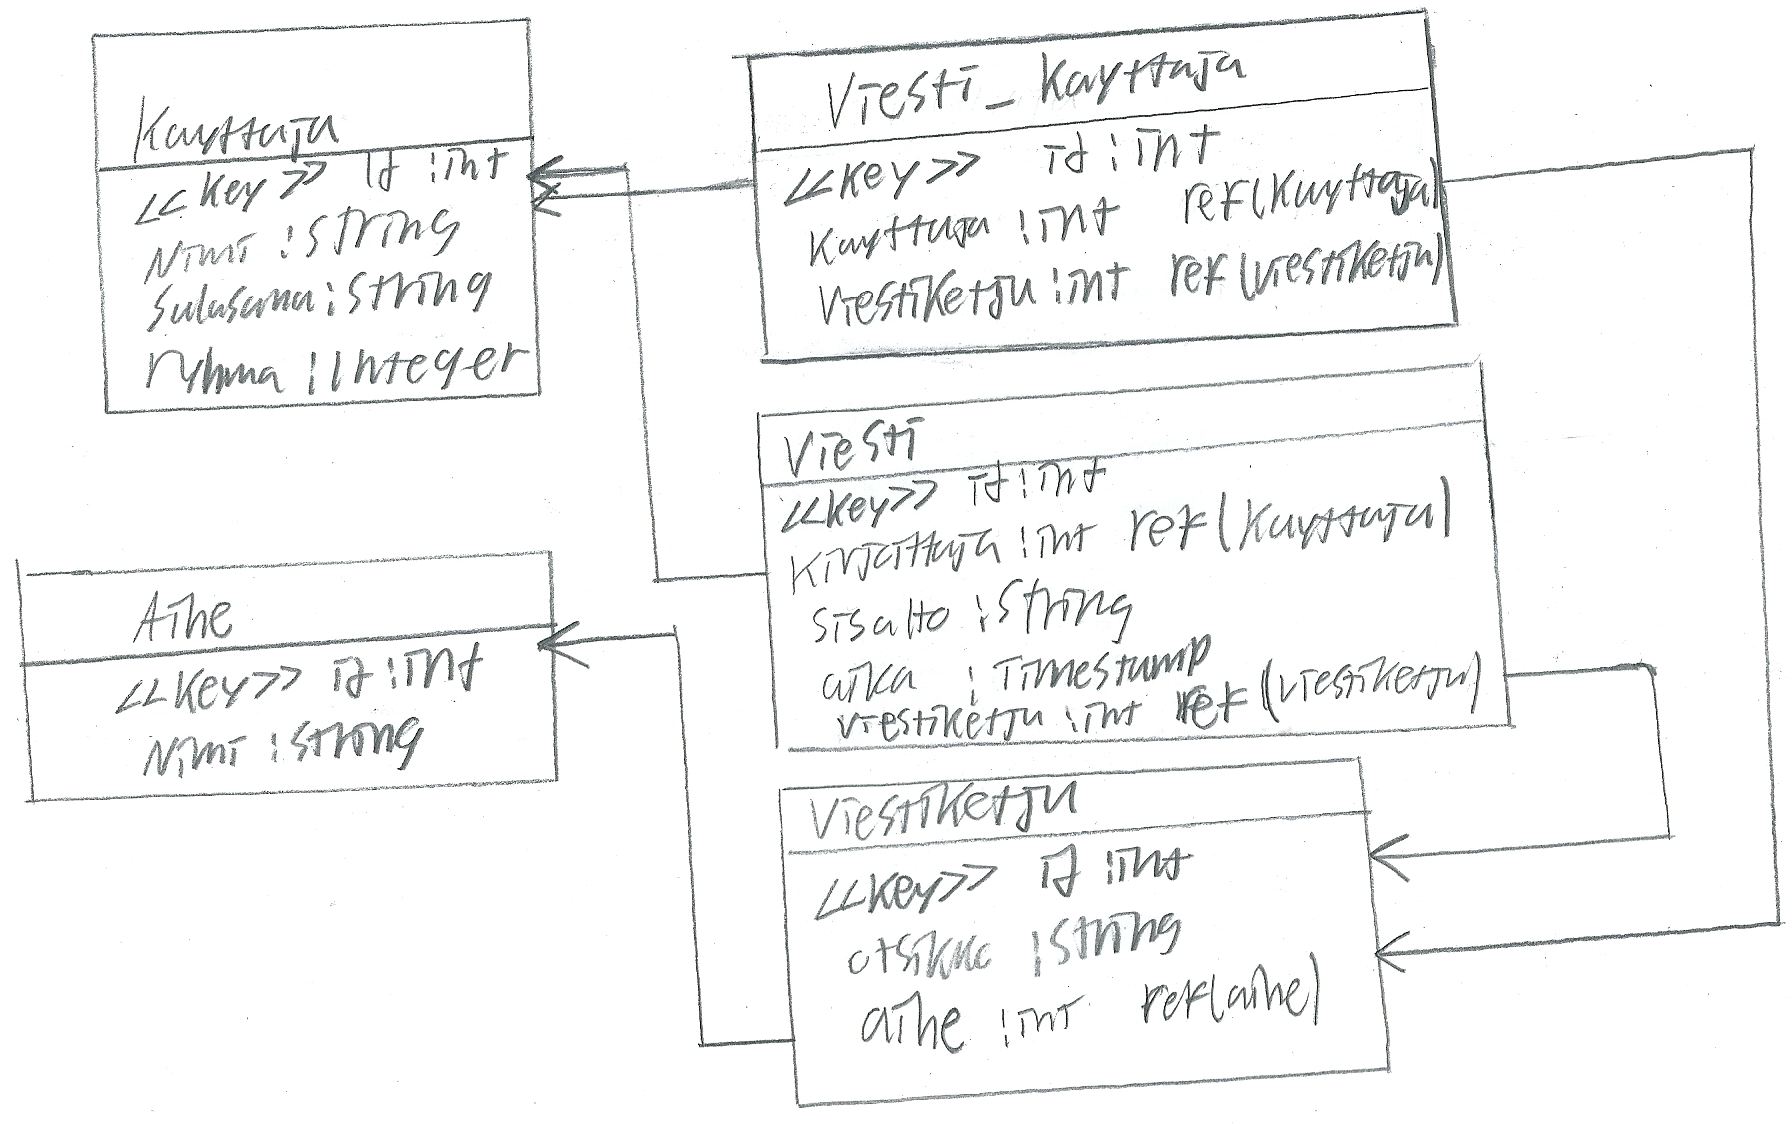
\includegraphics[width=\textwidth,height=\textheight,keepaspectratio]{relaatiotietokantakaavio.png}

\newpage

\section{Käyttöliittymä}
\subsection{Sivukartta}
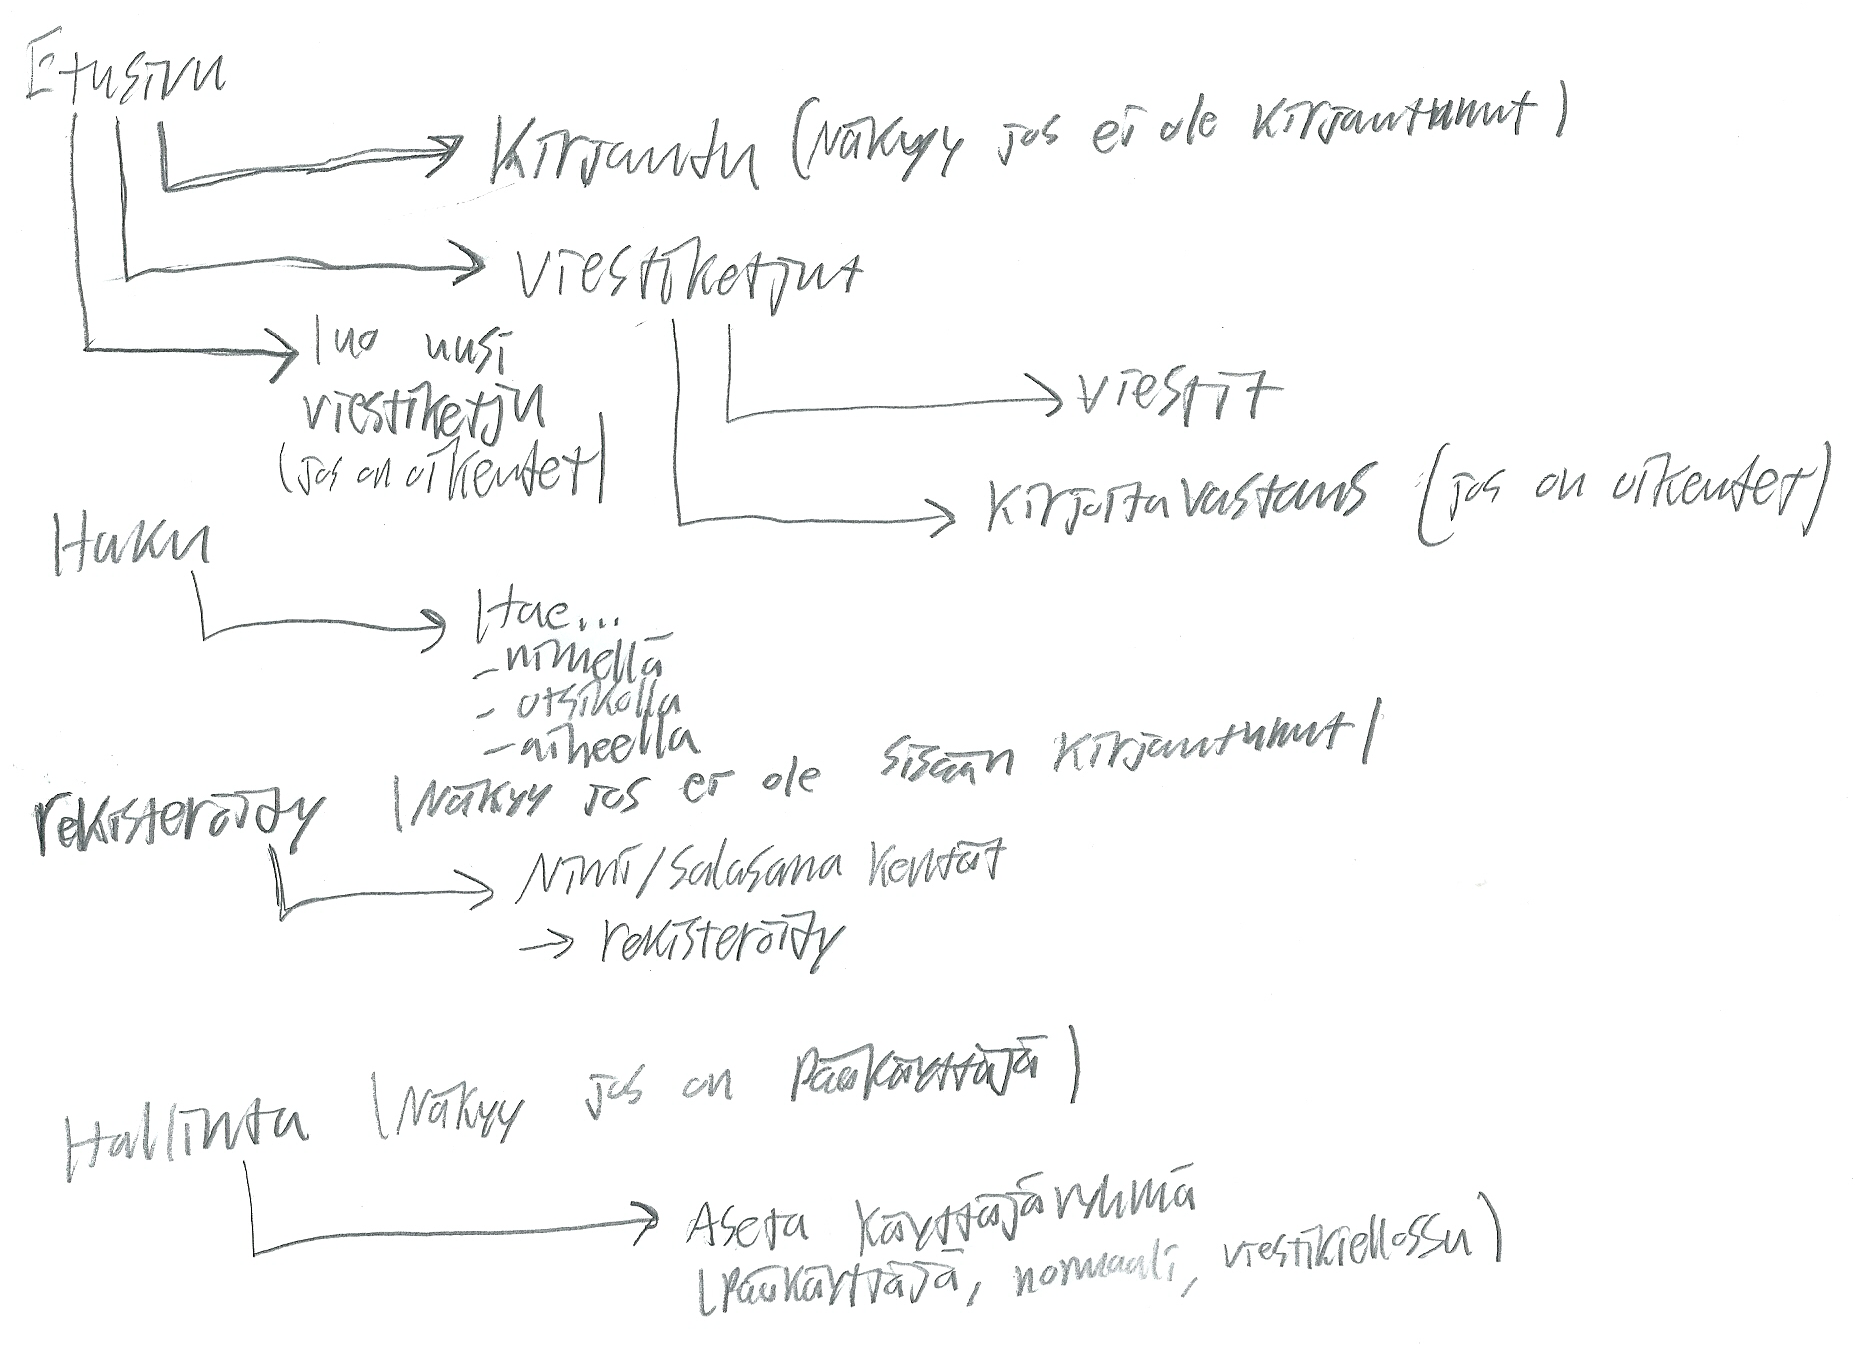
\includegraphics[width=\textwidth,height=\textheight,keepaspectratio]{kayttoliittymakaavio.png}

\subsection{Etusivu}
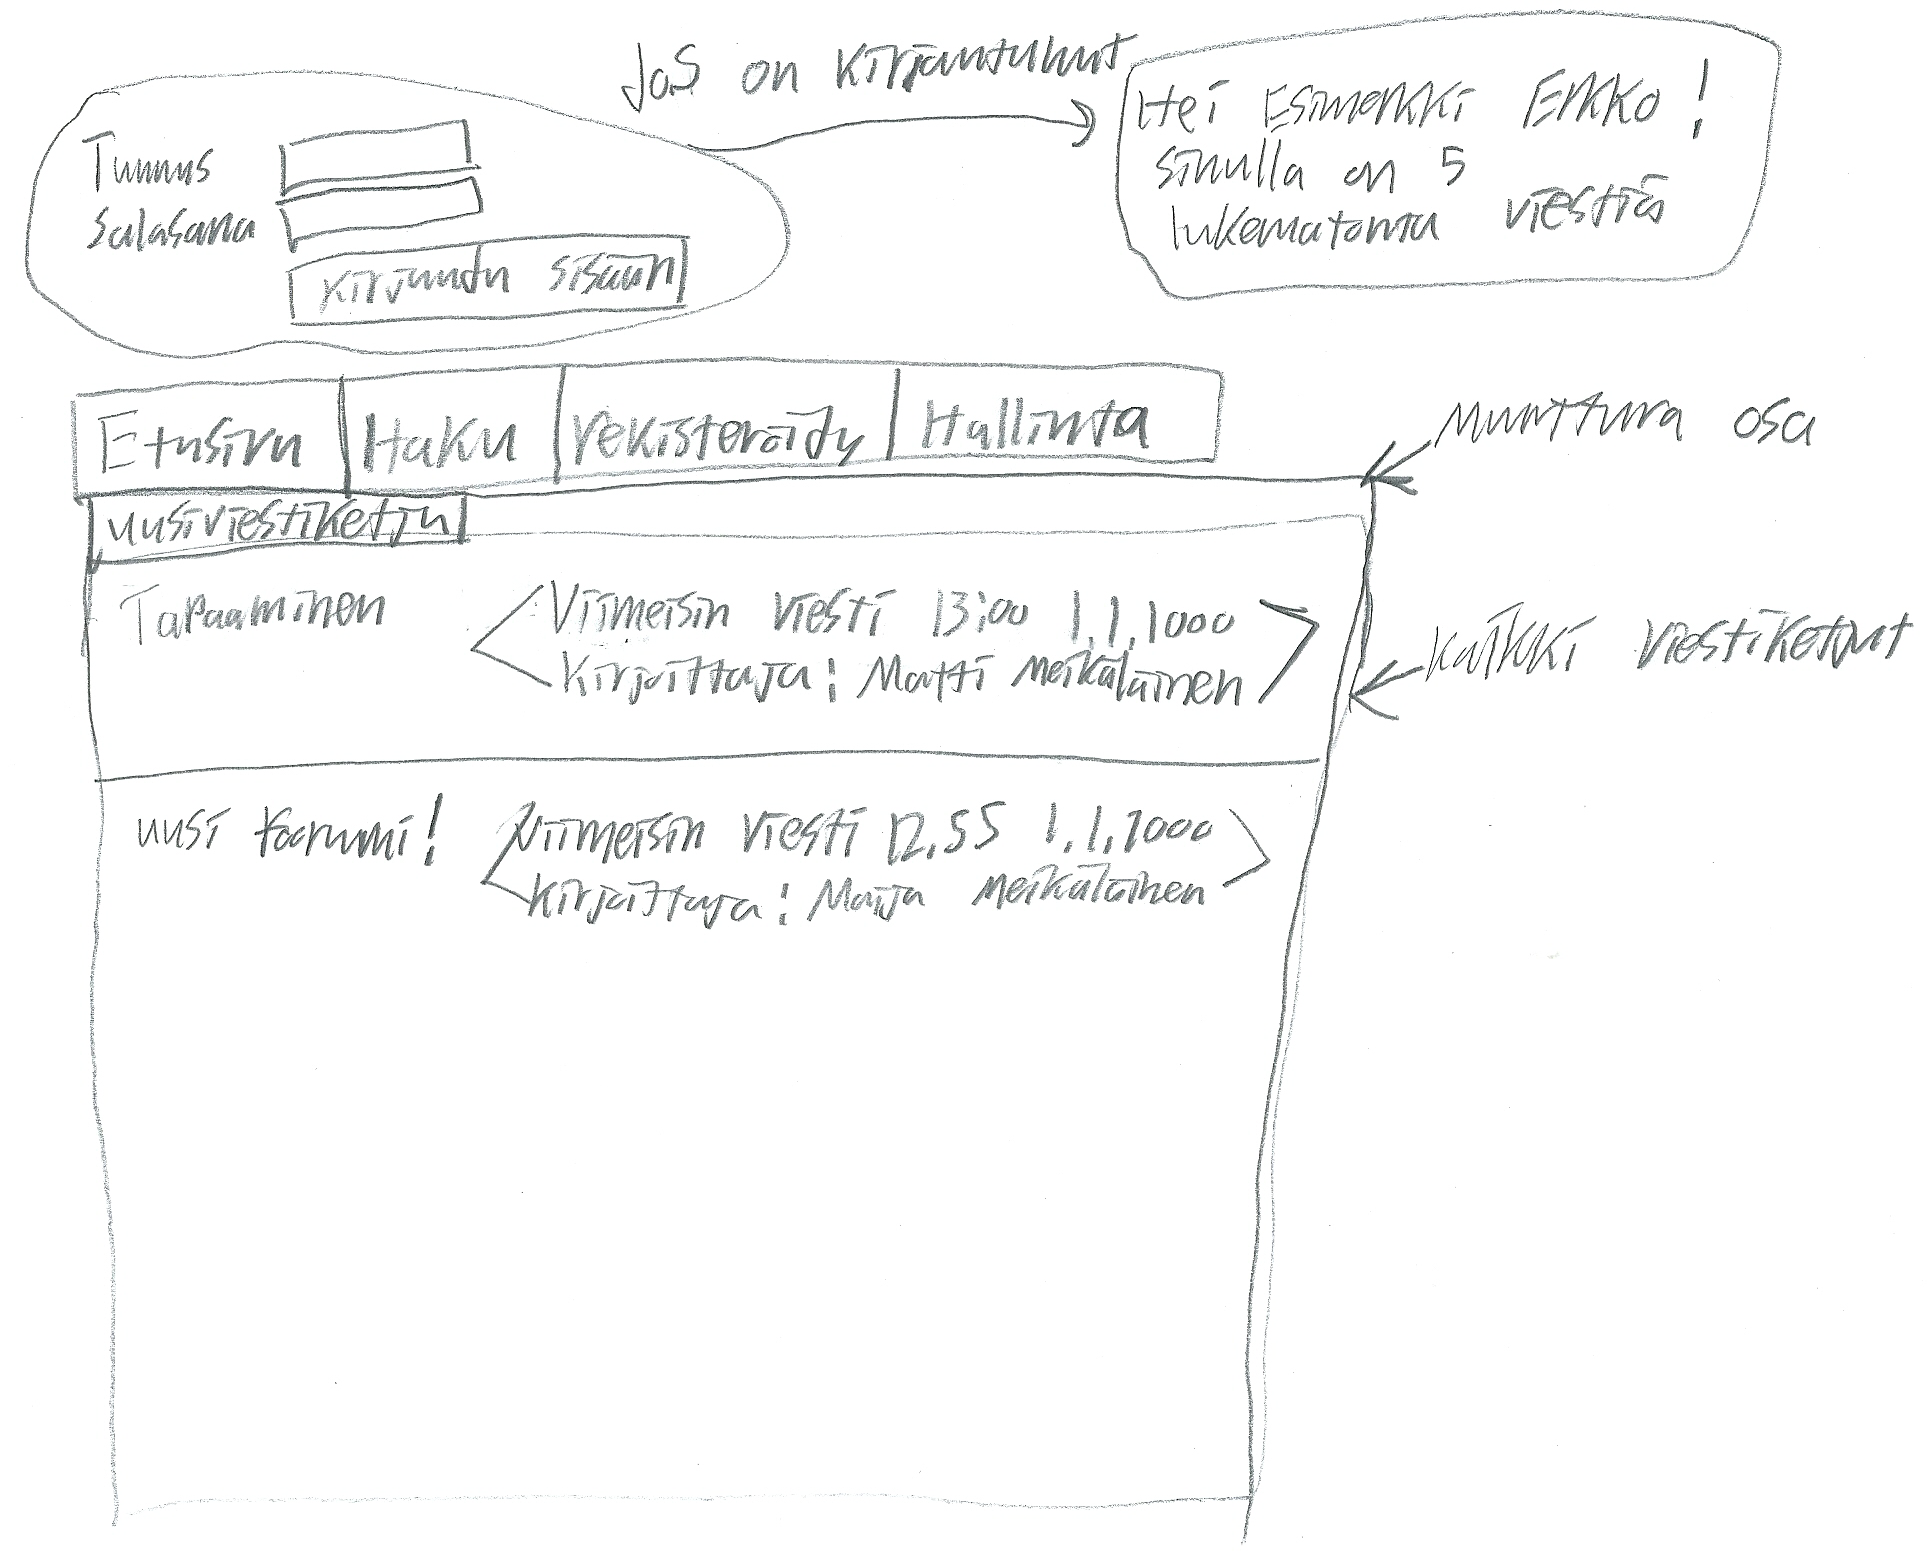
\includegraphics[width=\textwidth,height=\textheight,keepaspectratio]{etusivu.png}

\subsection{Haku}
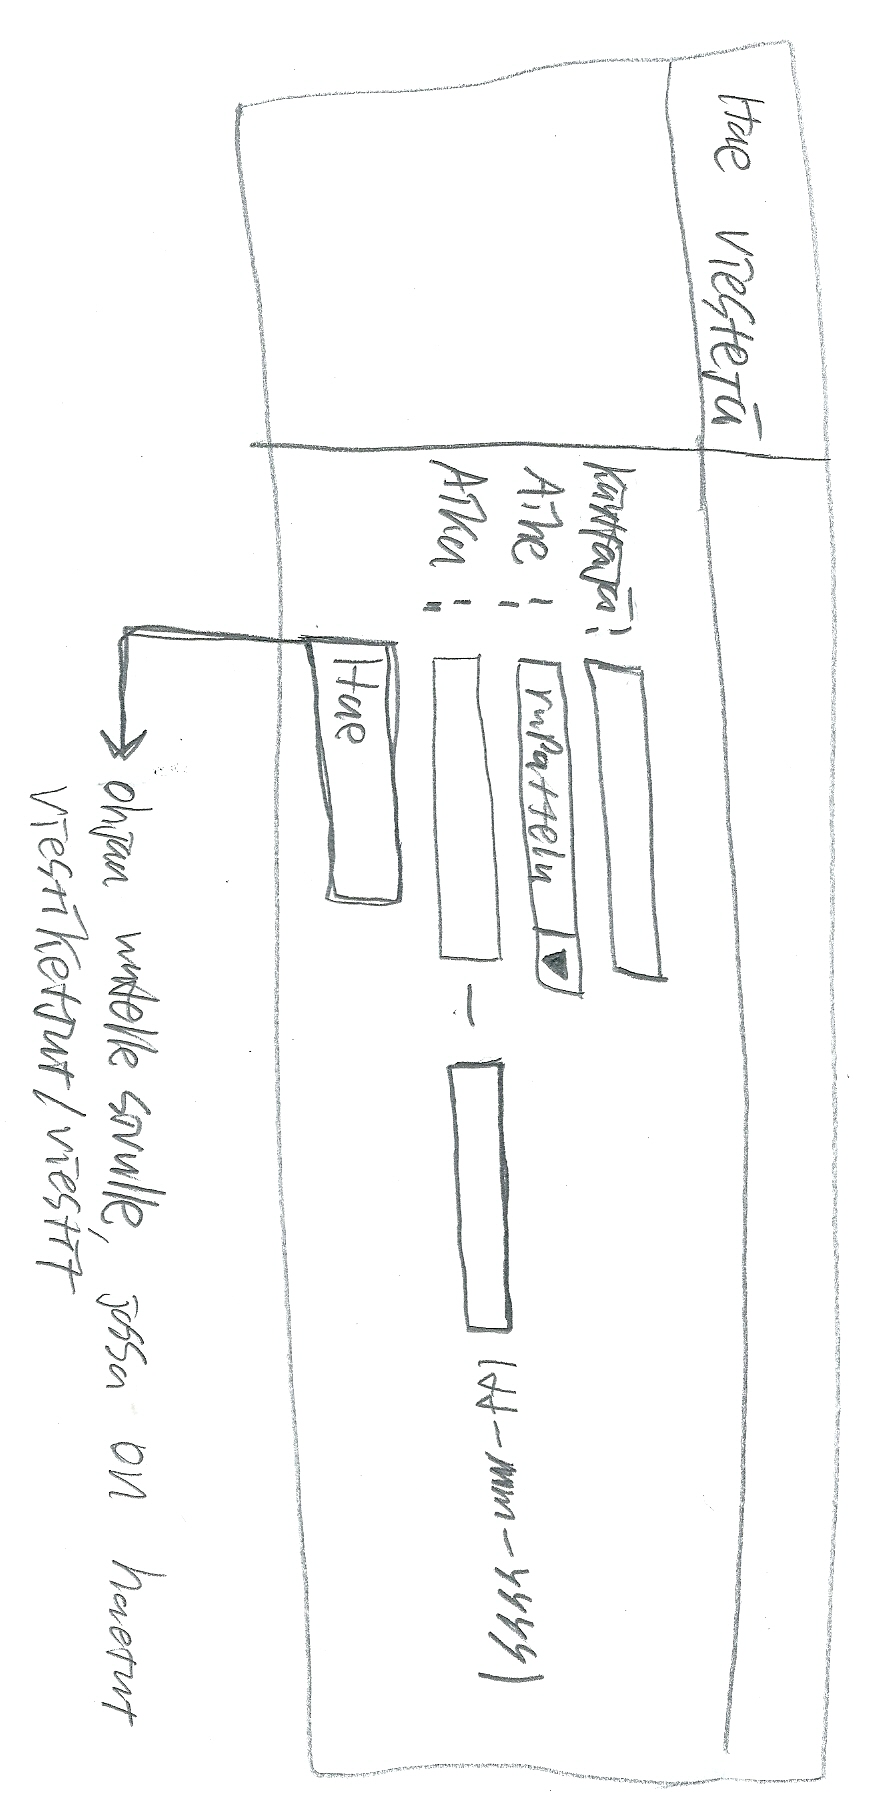
\includegraphics[width=\textwidth,height=\textheight,keepaspectratio]{haku.png}

\subsection{Hallinta}
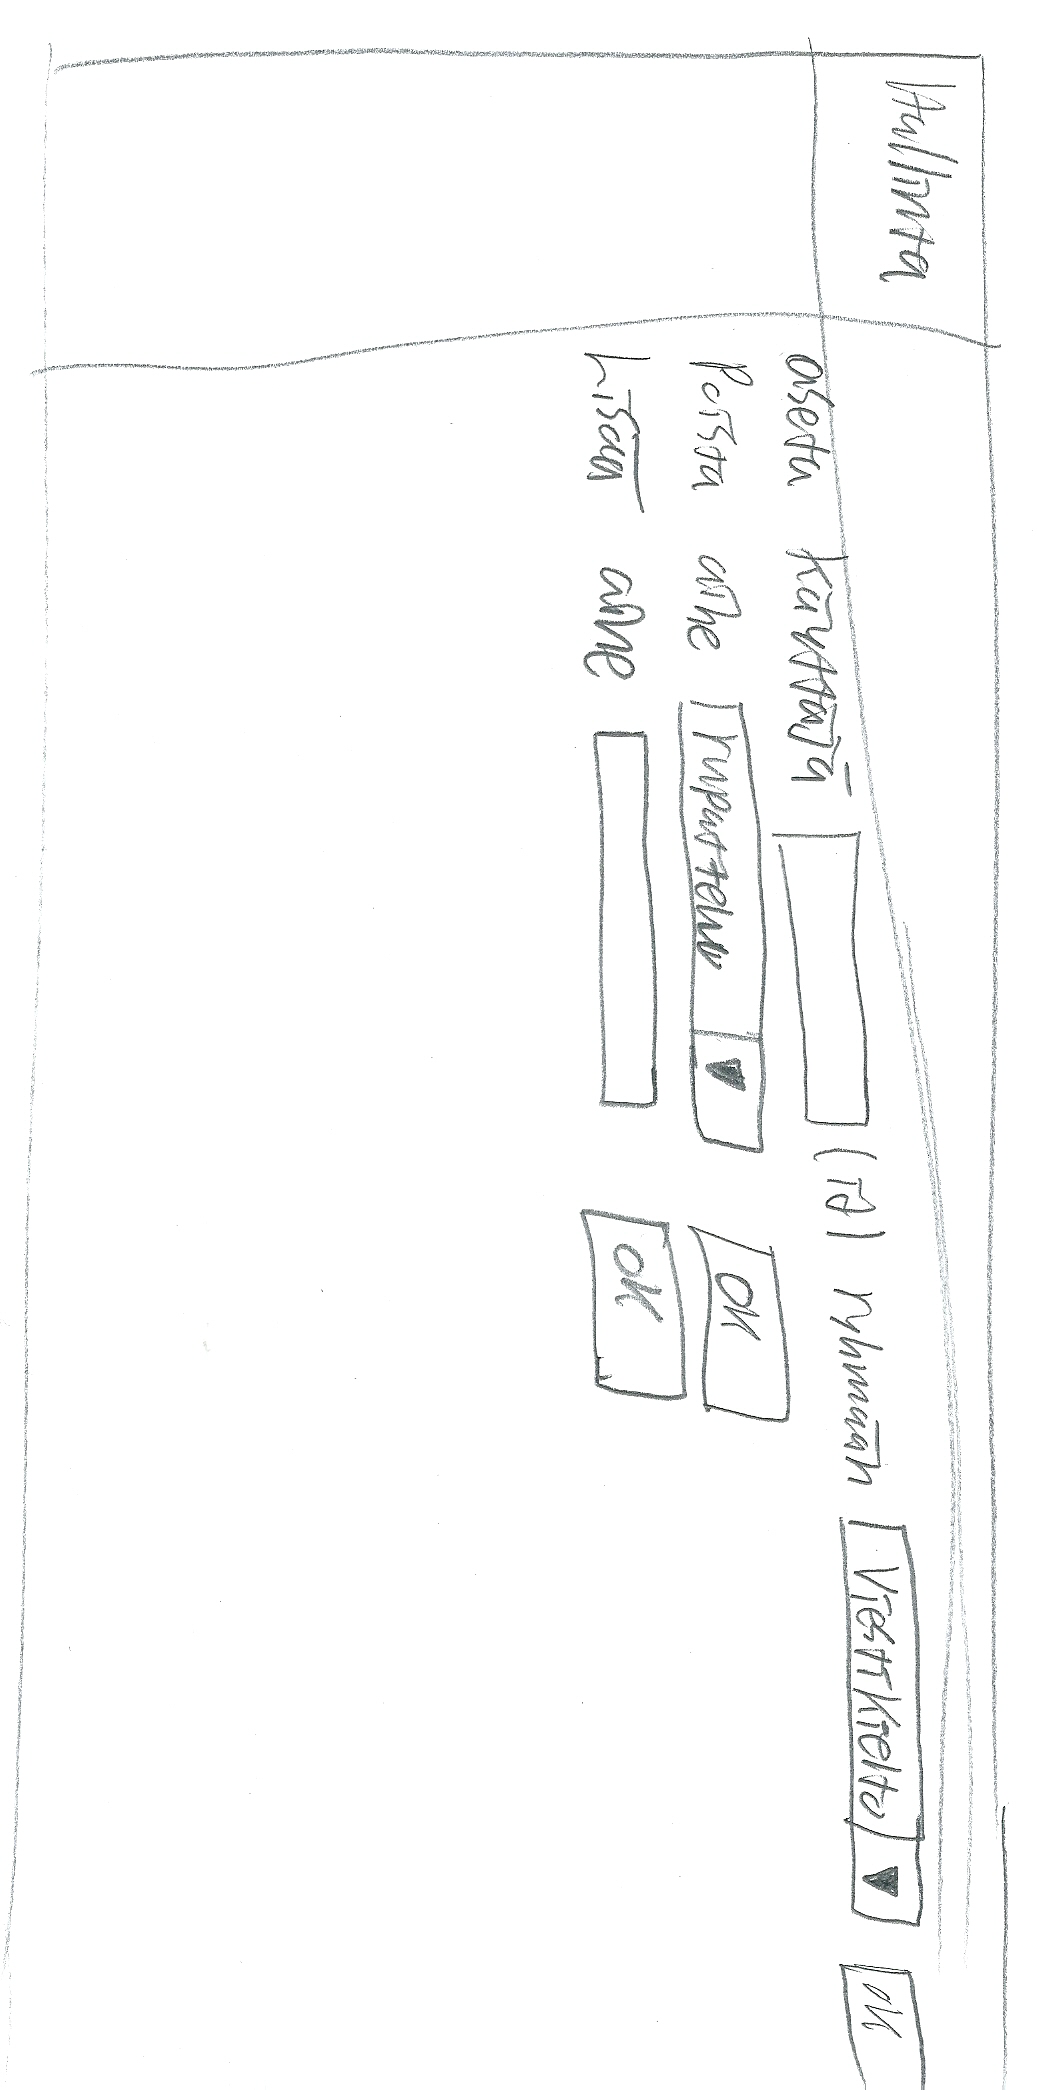
\includegraphics[width=\textwidth,height=\textheight,keepaspectratio]{hallinta.png}

\subsection{Rekisteröityminen}
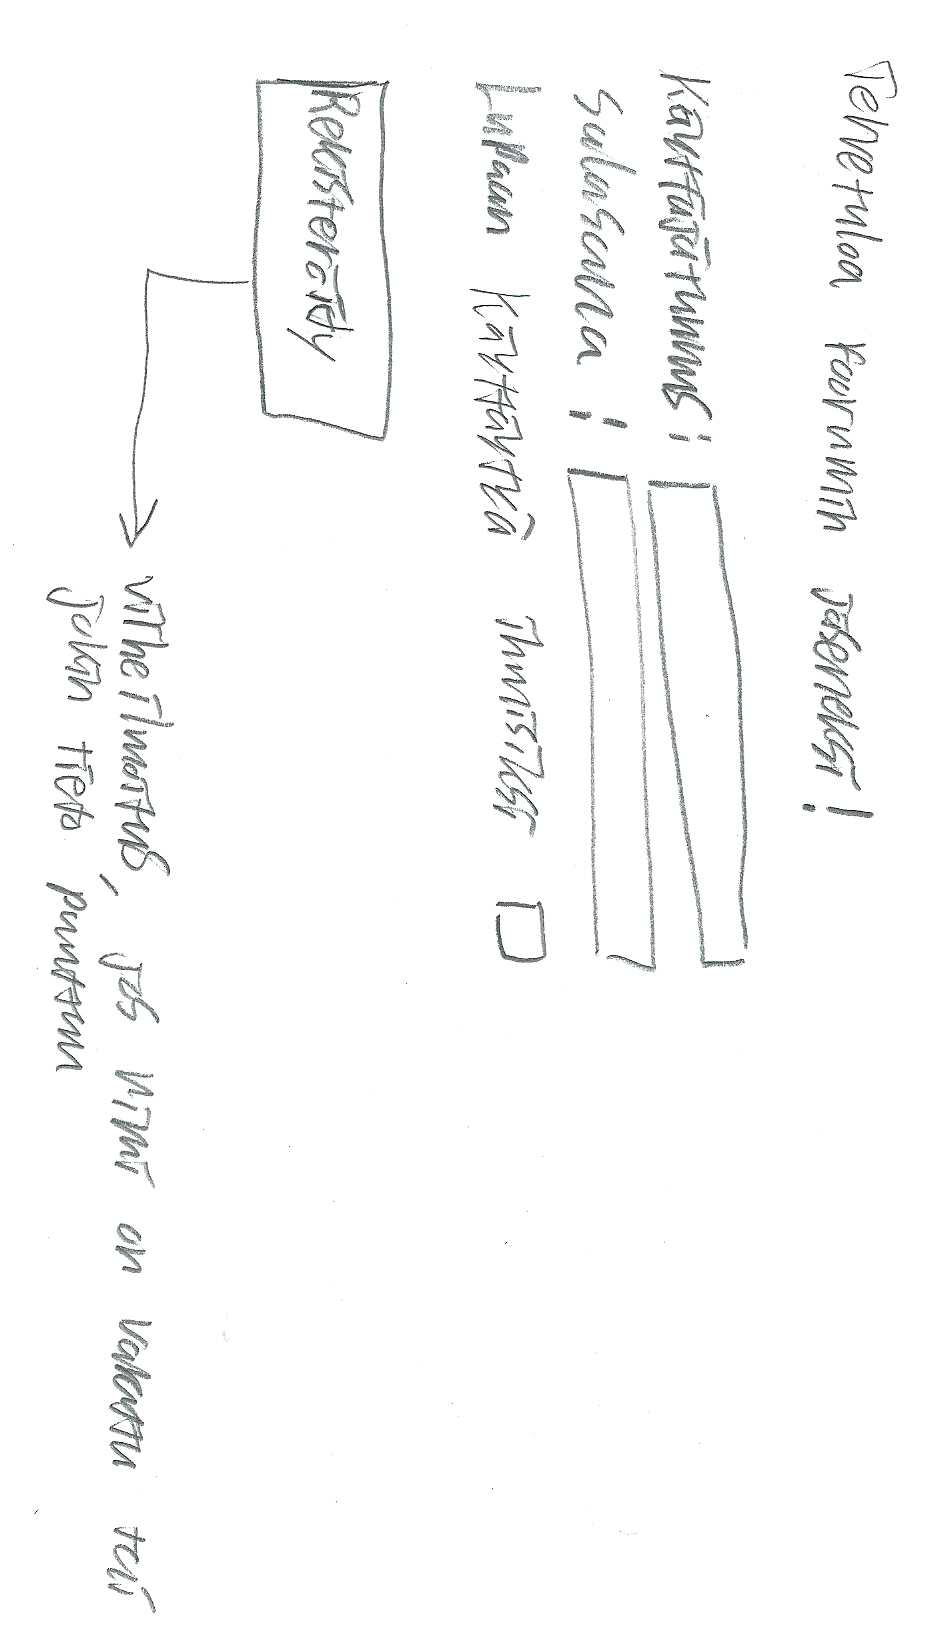
\includegraphics[width=\textwidth,height=\textheight,keepaspectratio]{rekisteroityminen.png}

\subsection{Uusiketju}
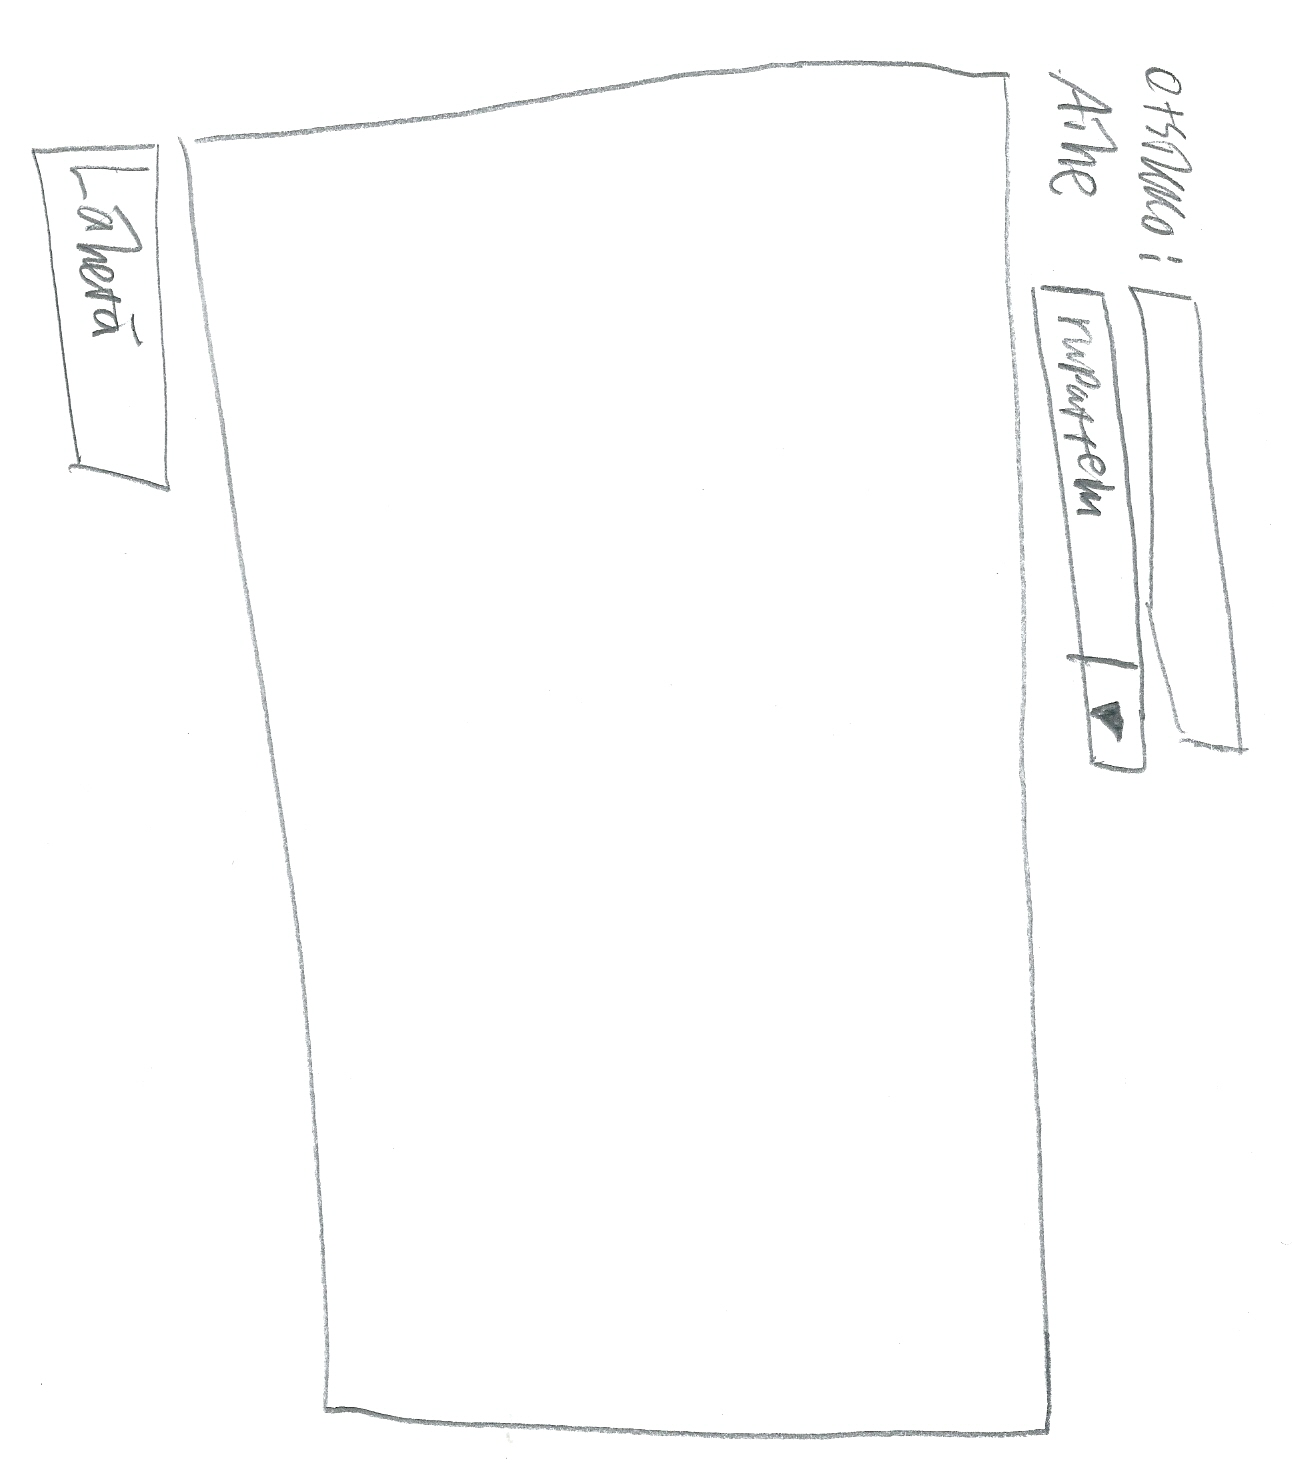
\includegraphics[width=\textwidth,height=\textheight,keepaspectratio]{uusiketju.png}

\subsection{Viestiketju}
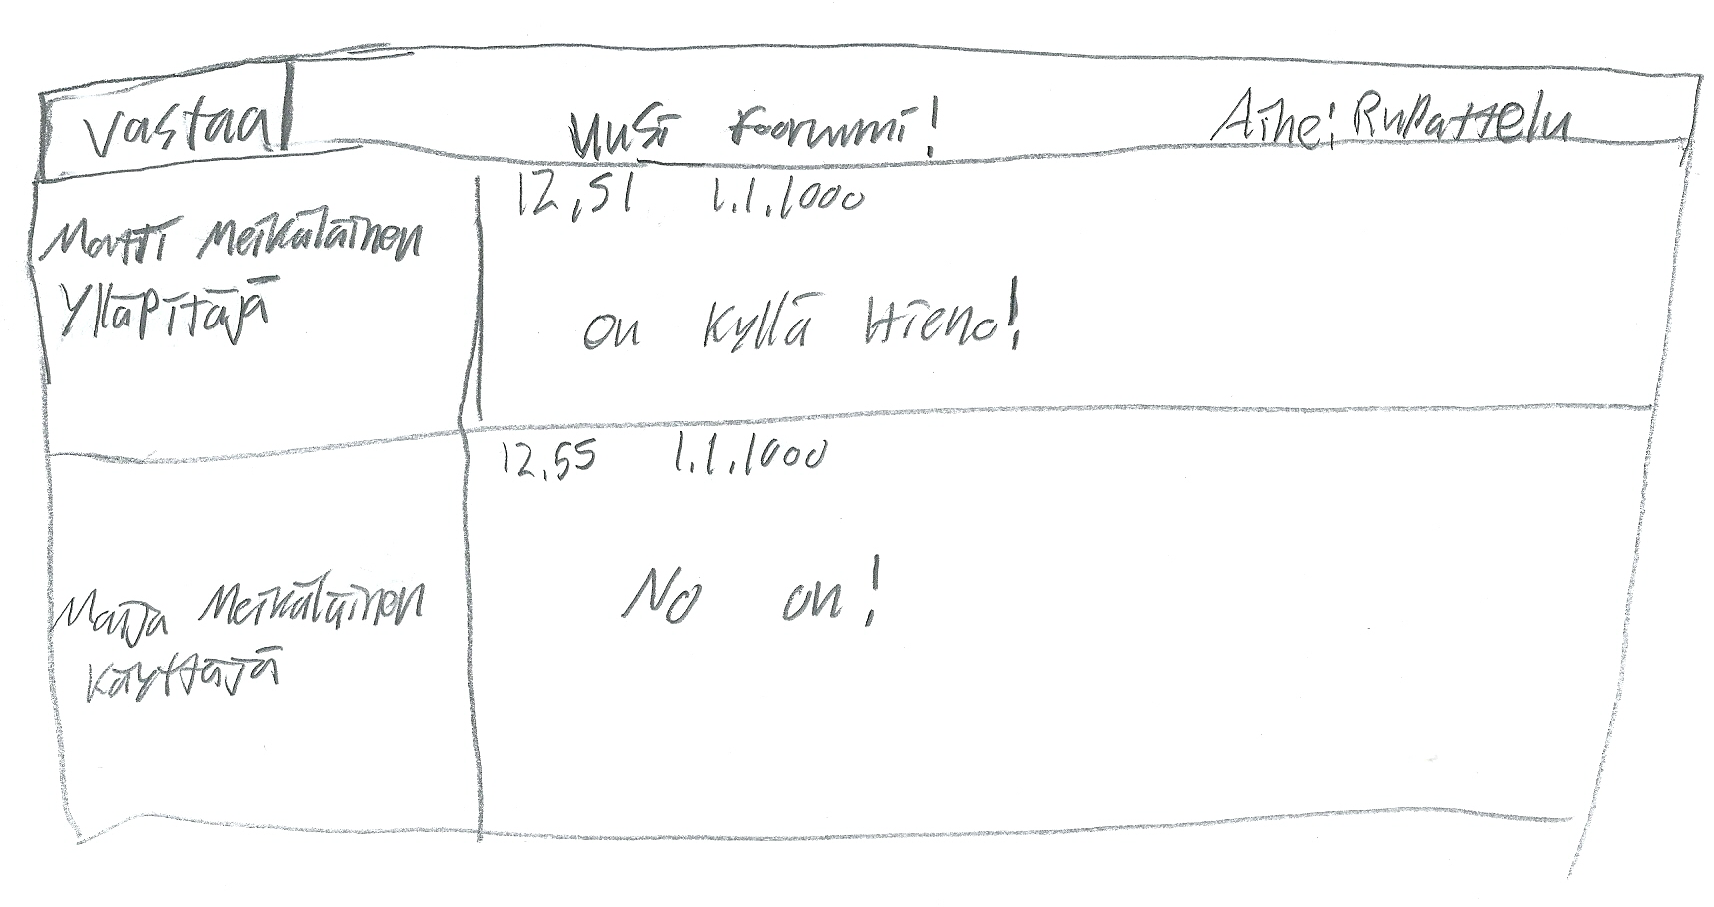
\includegraphics[width=\textwidth,height=\textheight,keepaspectratio]{viestiketju.png}

\subsection{Vastaus}
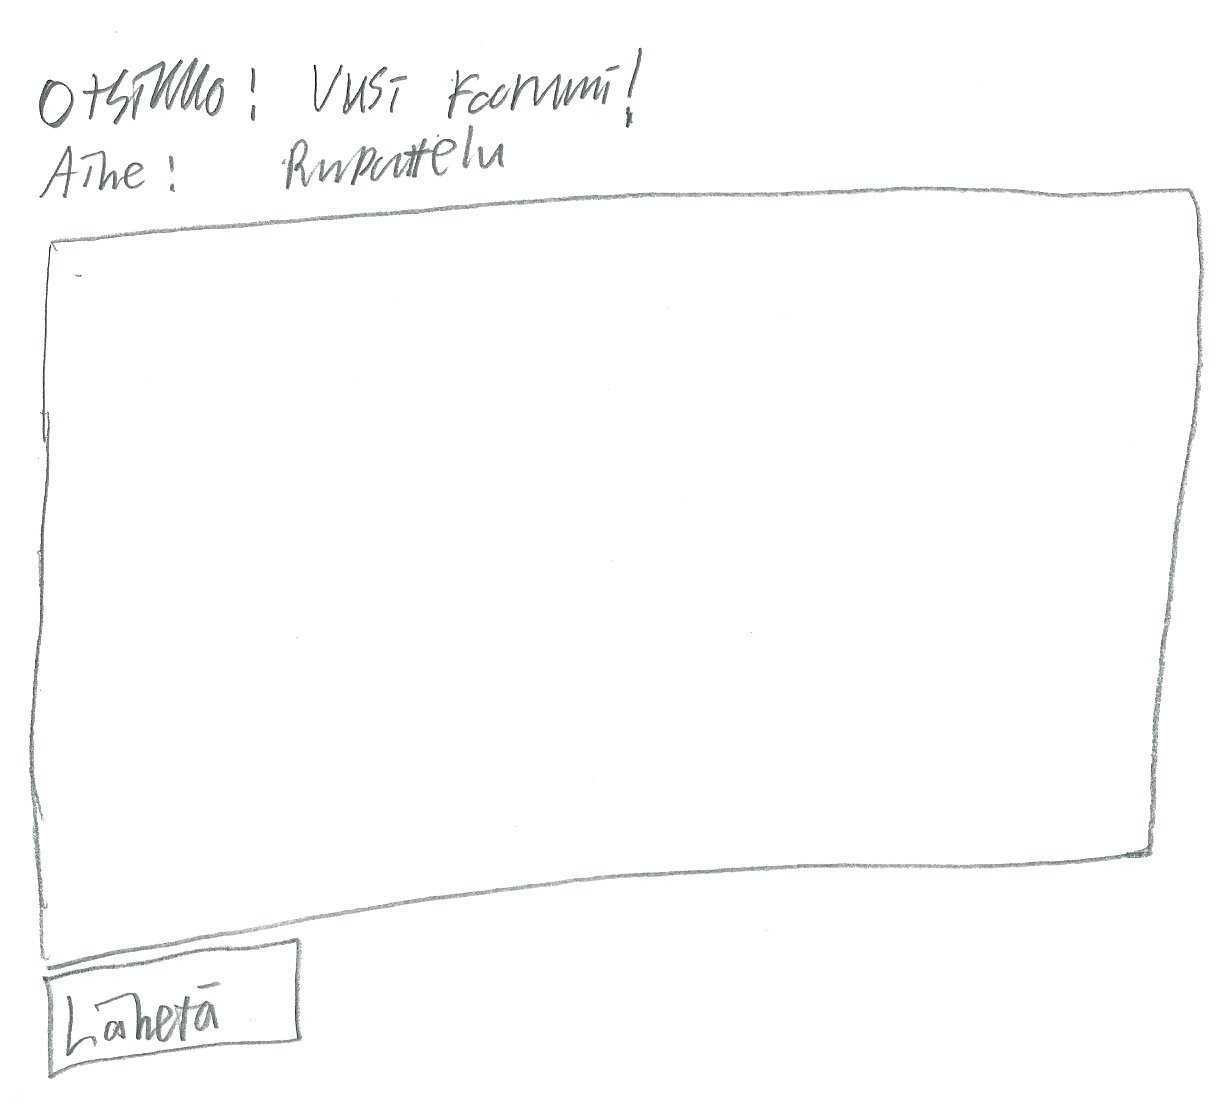
\includegraphics[width=\textwidth,height=\textheight,keepaspectratio]{vastaus.png}

\newpage

\section{Asennustiedot}
Foorumi on testattu PostgreSQL tietokannalla 8.4 sekä php 5.3:lla.
Foorumin asennus toteutetaan kopioimalla tiedostot johonkin näkyvään paikkaan, esimerkiksi kansioon htdocs.
Mitään salasanoja ei travitse laittaa, vaan users -palvelimella yhteys muodostetaan automaattisesti.
Kansiossa foorumi/sql on sql scriptit, joista osa pitää suorittaa ennen palvelimen käyttöönottoa.
create-tables.sql on pakollinen, jota ilman foorumi ei toimi lainkaan.
add-test-data.sql on valinnainen, nopeaa testausta varten.
Scripti luo roskatietoa.
Tällä hetkellä sitä kuitenkin tarvitaan, jos haluaa pääkäyttäjän oikeudet.
drop-tables.sql tuhoaa tietokannan sisällön. Tämän jälkeen tulee create-tables.sql suorittaa uudelleen.

\newpage

\section{Käyttöohjeet}
\begin{table}[ht]
\caption{Foorumin testitunnukset}
\centering
\begin{tabular}{c|c|c}
\hline
Nimi & Salasana & Rooli \\ [0.5ex]
\hline
NormiKäyttäjä&12345&Käyttäjä \\
Admin&admin&Ylläpitäjä \\
Käyttäjäkiellossa&666&Viestikiellossa \\ [1ex]
\hline
\end{tabular}
\end{table}

Kirjautuminen tapahtuu laittamalla tunnukset sivun yläosassa olevaan kirjautumislaatikkoon.
Kirjauduttua sisälle, käyttäjätunnuksen ja roolin tulisi näkyä kirjautumislaatikon tilalla.
Tällä hetkellä vain viestiketjuilla on täysi CRUD setti.
Niitä voi katsoa kuka tahansa ja niitä voivat rekisteröityneet käyttäjät luoda.
Ylläpitäjä voi muokata viestiketjujen aihetta tai otsikkoa.
Ylläpitäjä voi myös poistaa kokonaisia ketjuja.
Vaihtoehdot siihen tulevat viestikejun oikealle puolelle etusivulla.
Viestiketjuihin voi myös vastata.
Ylläpitäjä voi määritellä uusia aiheita ja poistaa vanhoja, olettaen että niihin ei liity viestiketjuja.
Hän voi myös asettaa käyttäjiä eriryhmiin.
Rekisteröitymällä pääsee käyttäjäryhmään.
Haku vaatii kaikkien arvojen asettamista, eli sekä päiväys että käyttäjän nimi tulee olla.
Päiväyksen ekaan kenttään tulee aikaisempi päiväys toiseen myöhempi.
Viestit palautetaan niiden väliltä.

\newpage

\section{Järjestelmän yleisrakenne}
Järjestelmä on toteutettu MVC-mallin mukaisesti.
Controlleri on kaikkien sivujen yhteinen, mutta jokaisella sivulla on omia toimintoja jotka kuuluvat niiden omille sivuille.
Yleisesti yksittäisiltä sivuilta siirretään tieto array:ssa controllerille, mutta tällä hetkellä osa datasta luodaan vasta kontrollerissa.
Controller luo pohjasivusta ilmentymän, johon liitetään kysytty sivu.
Kaikki tietokantayhteydet ovat vain tietokantayhteys.php:ssa.
Käyttäjäoikeudet ovat models/groups kansiossa.
Tietokantamallit ovat models kansiossa.
Istuntoon tallennetaan käyttäjän kirjautuminen, virhe- ja onnistumisviestit.
Virhe- ja onnistumisviestit poistetaan istunnosta näytön jälkeen.
Kirjautuminen säilyy niin kauan kunnes käyttäjä kirjautuu ulos tai selain poistaa sen.
Malli luokat ovat toteutettu siten, että niitä luodaan staattisilla metodeilla.
Samoin toimii niiden muuttujien tallennus.
Käyttäjäryhmät toteuttavat kaikki ryhma interfacen.
Jokainen käyttäjäryhmä luokka toteuttaa käyttöoikeuksia virtuaalisilla metodeilla, sekä sivujen katsomisoikeudet arraylla.
Sivujen katsomisoikeudet toimivat siten, että ellei erikseen ole ryhmälle lupaa nähdä sivua, sitä ei näytetä.

\newpage

\section{Käyttöliittymä ja järjestelmän komponentit}
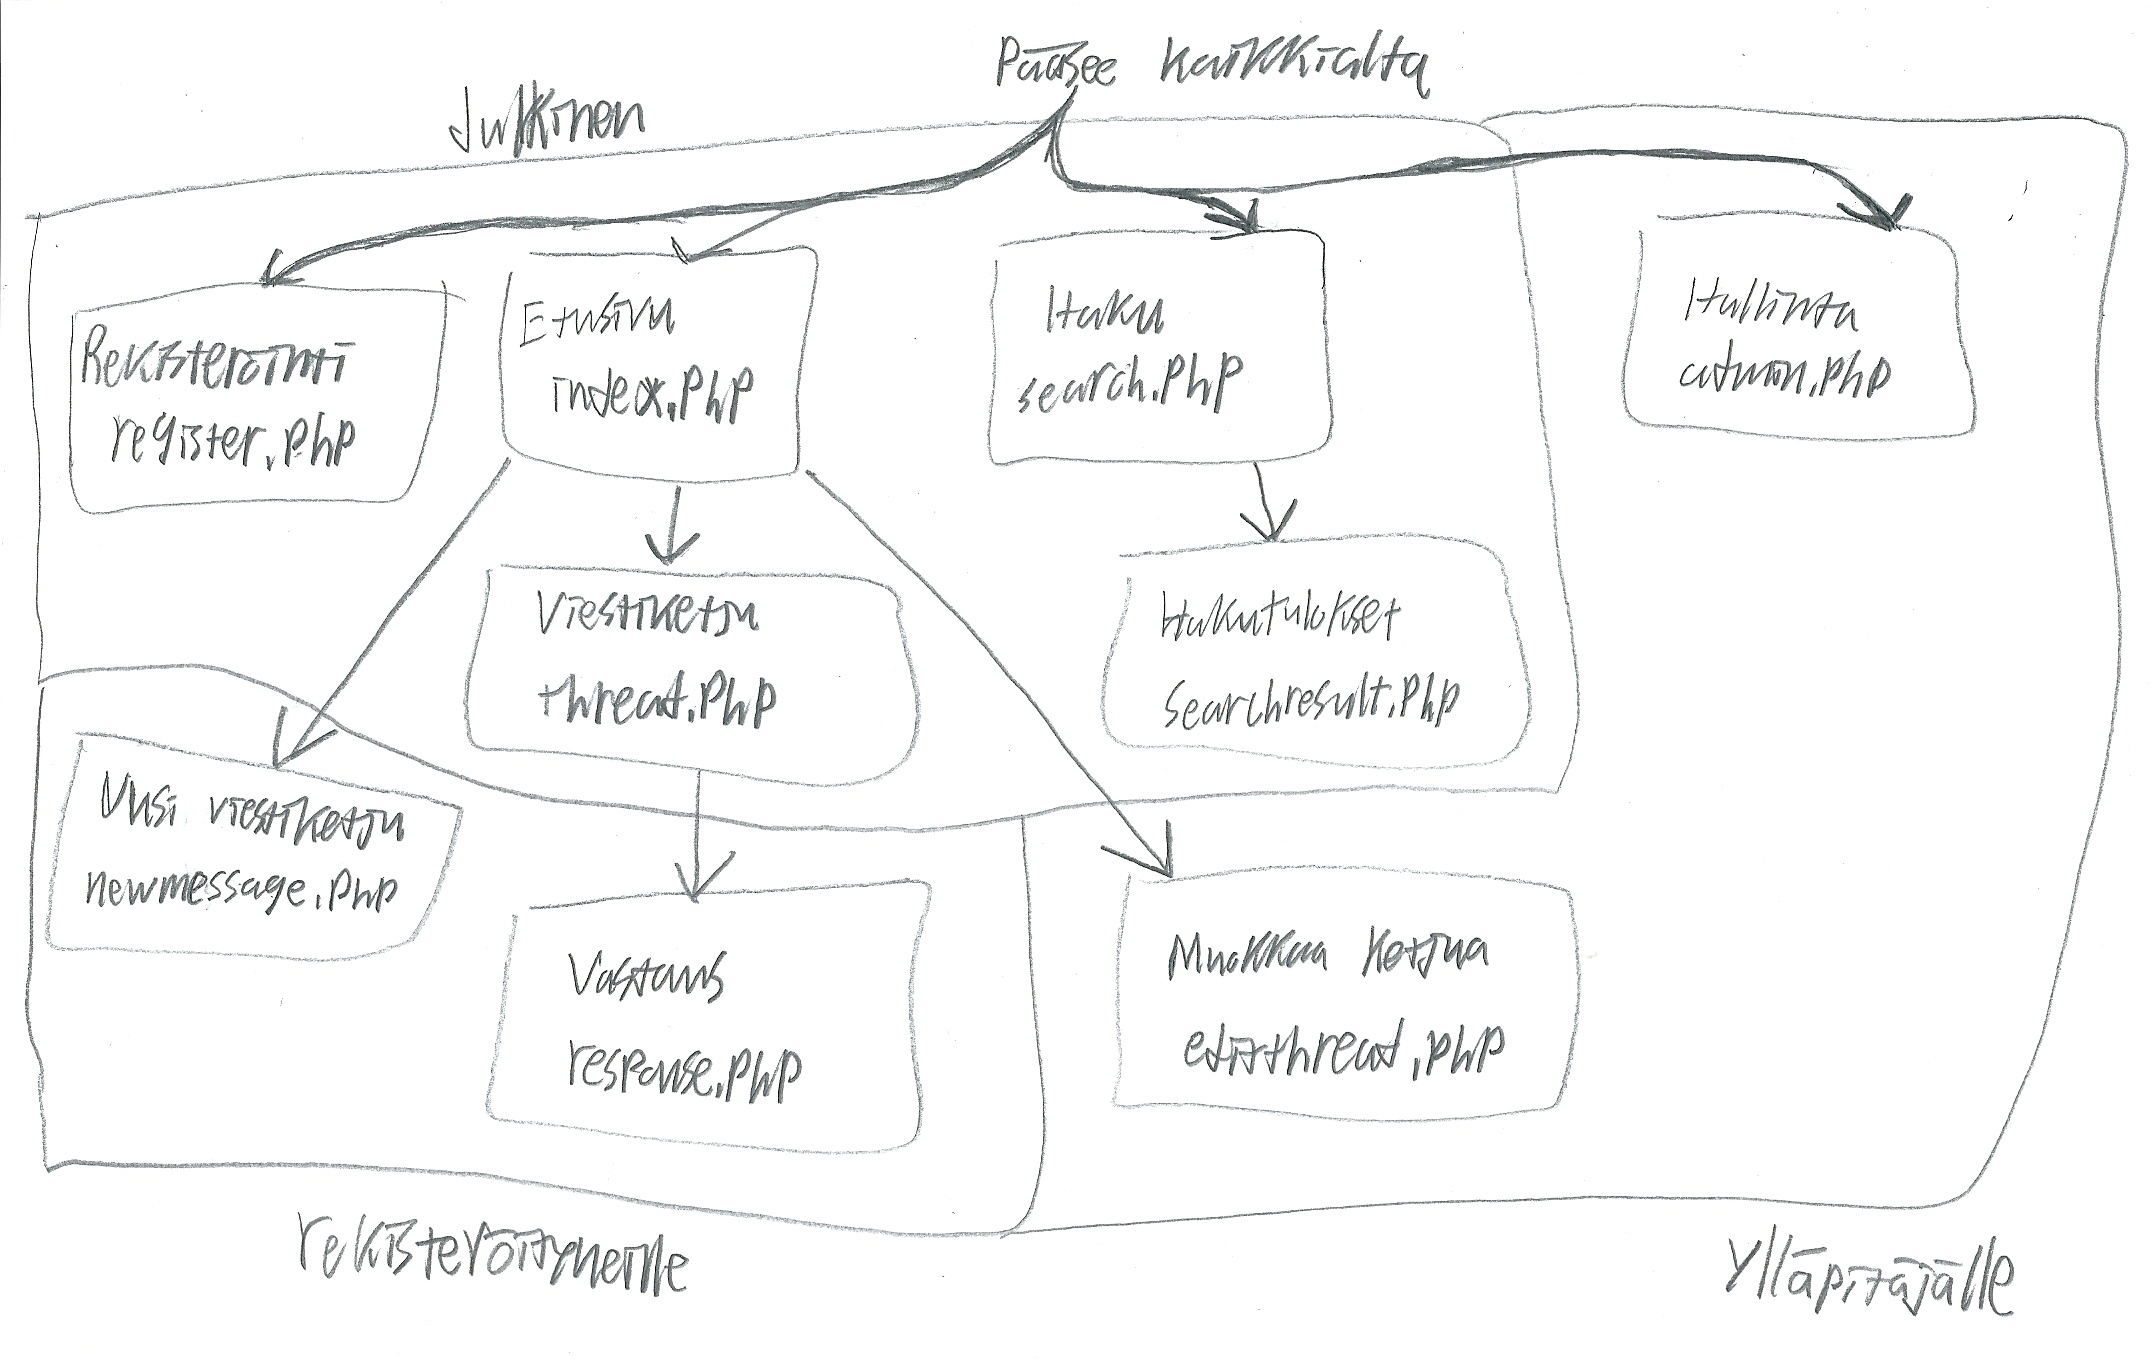
\includegraphics[width=\textwidth,height=\textheight,keepaspectratio]{kayttoliittyma.png}

\end{document}
